\documentclass[Orbiter User Manual.tex]{subfiles}
\begin{document}

\section{Spacecraft controls}
\label{sec:controls}
This chapter contains guidelines on how to control your spacecraft in free space (outside the influence of aerodynamic forces induced by a planetary atmosphere). We are considering a "generic" vessel with a standard engine layout. The handling of individual spacecraft types may vary considerably. Always read the operating instructions of your vessel, if available.

\subsection{Main, retro and hover engines}
Main thrusters accelerate the ship forward, \textit{retro thrusters} (if installed) accelerate it backward. Main and retro thrusters can be adjusted with \Ctrl\keystroke{+}$_{Num}$ (to increase main thrust of decrease retro thrust) and \Ctrl\keystroke{-}$_{Num}$ (to decrease main thrust or increase retro thrust). Main and retro thrusters can be killed with \Ctrl\keystroke{*}$_{Num}$. The permanent setting can be temporarily overridden with \keystroke{+}$_{Num}$ (set main thrusters to 100\%) and \keystroke{-}$_{Num}$ (set retro thrusters to 100\%). To set permanent full main thrust directly, press and hold \keystroke{+}$_{Num}$, followed by \Ctrl to lock the setting. If available, a joystick throttle control can be used to set the main thrusters.

\begin{table}[H]
	\centering
	\begin{tabular}{ |p{0.3\textwidth}|p{0.3\textwidth}|p{0.3\textwidth}| }
	\hline\rule{0pt}{2ex}
	\textbf{Main} & \textbf{Retro} & \textbf{Hover}\\
	\hline\rule{0pt}{2ex}
		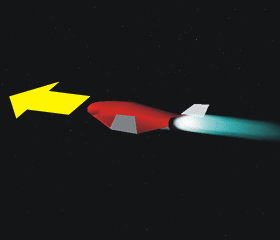
\includegraphics[width=0.3\textwidth, margin=0pt 1ex 0pt 1ex, valign=m]{control_main.png}
	&
		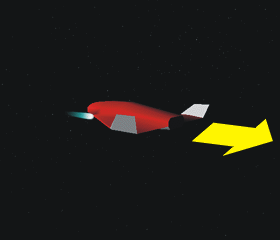
\includegraphics[width=0.3\textwidth, margin=0pt 1ex 0pt 1ex, valign=m]{control_retro.png}
	&
		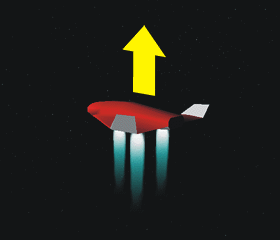
\includegraphics[width=0.3\textwidth, margin=0pt 1ex 0pt 1ex, valign=m]{control_hover.png}
	\\
	\hline\rule{0pt}{2ex}
		\begin{itemize}[leftmargin=*]
		\item \Ctrl\keystroke{+}$_{Num}$ (permanent)
		\item \keystroke{+}$_{Num}$ (temp. 100\%)
		\item Joystick throttle control
		\end{itemize}
	&
		\begin{itemize}[leftmargin=*]
		\item \Ctrl\keystroke{-}$_{Num}$ (permanent)
		\item \keystroke{-}$_{Num}$ (temp. 100\%)
		\end{itemize}
	&
		\begin{itemize}[leftmargin=*]
		\item \keystroke{0}$_{Num}$ (increase)
		\item \keystroke{.}$_{Num}$ (decrease)
		\end{itemize}
	\\
	\hline
	\end{tabular}
\end{table}

\noindent
\\
\textbf{Background: Rocket propulsion}\\
The ship's acceleration \textbf{a} resulting from engaging main or retro thrusters depends on the force \textbf{F} produced by the engines, and the ship's mass \textit{m}:

\[ \textbf{F} = m \, \textbf{a} \]

\noindent
Note that both \textbf{a} and \textbf{F} are vectors, that is, they have a direction as well as a magnitude. In the absence of additional forces (such as gravity or atmospheric drag) the spacecraft moves with constant velocity \textbf{v} as long as no engines are engaged. When the engines are firing, the resulting acceleration \textbf{a} changes the velocity according to

\[ \frac{d\textbf{v}(t)}{dt} = \textbf{a}(t) \]

\noindent
For a fixed thruster setting \textbf{F} the acceleration will slowly increase as fuel is consumed, resulting in a reduction of the ship's mass \textit{m}. This situation is described by the \textit{rocket equation}:

\[ m(t) \frac{d\textbf{v}(t)}{dt} = - \textbf{c} \frac{dm(t)}{dt} \]

\noindent
where thrust \textbf{F} = -\textbf{c} dm/dt is given by the product of exhaust velocity \textbf{c} and mass flow rate dm/dt. This can be integrated over a time interval to compute the change in velocity $\Delta$\textbf{v} as a function of initial mass $m_{0}$ and final mass $m_{1}$:


\[ \Delta \textbf{v} = \textbf{c} \ln \frac{m_{0}}{m_{1}} \]

\noindent
Hover engines, if available, are mounted underneath the ship's fuselage to provide upward thrust. Hover engines are typically used for \textit{spaceplane} designs to provide vertical take-off and landing (VTOL) capabilities without the need to tilt the ship upward to obtain a vertical acceleration component from the main thrusters. Standard rocket layouts ("tailsitters") don't have dedicated hover thrusters, because the main engines are used to produce the take-off (and sometimes landing) thrust. Hover thrust is increased with \keystroke{0}$_{Num}$ and decreased with \keystroke{.}$_{Num}$.\\
The current main/retro thruster setting and corresponding thrust [N] are shown in the engine control block in the top left corner of the generic glass cockpit view (MAIN ENG, see \ref{ssec:glass_cockpit}). The indicator bar is green for positive (main) thrust, and yellow for negative (retro) thrust. If applicable, the hover thrust setting (HOVR ENG) is also shown. Spacecraft which support customised instrument panel and virtual cockpit views usually have their own indicators for engine status displays.\\
The maximum vacuum thrust ratings for main, retro and hover thrusters, as well as the current spacecraft mass, are displayed in the vessel's info sheet (\Ctrl\keystroke{I}). Values are in Newton (1 N = 1 kg m s$^{-2}$). Note that the actual generated thrust may be lower in the presence of ambient atmospheric pressure. At extremely high atmospheric pressures, e.g. on the surface of Venus, the spacecraft engines may not produce any thrust at all.


\subsection{Attitude thrusters}
\label{ssec:control_att}
Attitude thrusters are small engines which are engaged in pairs to change the angular velocity of the spacecraft around a specific axis by generating an angular momentum. A complete set of attitude thrusters that allows to control the vessel's orientation in all three of its principal axes is often referred to as \textit{reaction control system} (RCS). The same set of thrusters, fired in different configurations, may also be used to generate linear thrust for acceleration along its principal axes without changing the vessel's orientation.\\
In Orbiter, the RCS mode is set to either rotational (ROT) or linear (LIN) with \keystroke{/}$_{Num}$. The RCS can also be disabled (OFF) with \Ctrl\keystroke{/}$_{Num}$, for example during launch, where attitude is more commonly controlled by gimballing the main engines, or during reentry, where body shape or aerodynamic surfaces control flight attitude. The current mode is shown in the engine display block in the top left of the glass cockpit view.\\
Attitude thrusters are controlled with the keyboard or joystick. In rotational mode:

\begin{table}[H]
	\centering
	\begin{tabular}{ |p{0.3\textwidth}|p{0.3\textwidth}|p{0.3\textwidth}| }
	\hline\rule{0pt}{2ex}
	\textbf{Rotate: yaw} & \textbf{Rotate: pitch} & \textbf{Rotate: roll}\\
	\hline\rule{0pt}{2ex}
		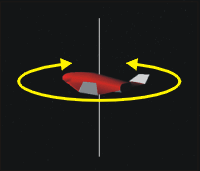
\includegraphics[width=0.3\textwidth, margin=0pt 1ex 0pt 1ex, valign=m]{control_yaw.png}
	&
		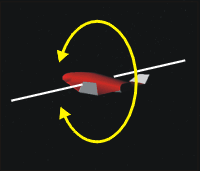
\includegraphics[width=0.3\textwidth, margin=0pt 1ex 0pt 1ex, valign=m]{control_pitch.png}
	&
		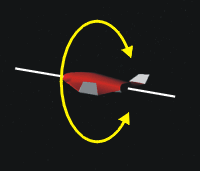
\includegraphics[width=0.3\textwidth, margin=0pt 1ex 0pt 1ex, valign=m]{control_roll.png}
	\\
	\hline\rule{0pt}{2ex}
		\begin{itemize}[leftmargin=*]
		\item \keystroke{1}$_{Num}$ / \keystroke{3}$_{Num}$
		\item Joystick rudder control
		\item Joystick left/right+Button 2
		\end{itemize}
	&
		\begin{itemize}[leftmargin=*]
		\item \keystroke{2}$_{Num}$ / \keystroke{8}$_{Num}$
		\item Joystick forward/back
		\end{itemize}
	&
		\begin{itemize}[leftmargin=*]
		\item \keystroke{4}$_{Num}$ / \keystroke{6}$_{Num}$
		\item Joystick left/right
		\end{itemize}
	\\
	\hline
	\end{tabular}
\end{table}

\noindent
and in linear (translational) mode:

\begin{table}[H]
	\centering
	\begin{tabular}{ |p{0.3\textwidth}|p{0.3\textwidth}|p{0.3\textwidth}| }
	\hline\rule{0pt}{2ex}
	\textbf{Translate: forward/back} & \textbf{Translate: left/right} & \textbf{Translate: up/down}\\
	\hline\rule{0pt}{2ex}
		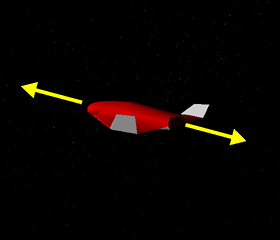
\includegraphics[width=0.3\textwidth, margin=0pt 1ex 0pt 1ex, valign=m]{control_fwd_back.png}
	&
		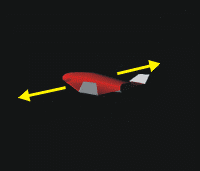
\includegraphics[width=0.3\textwidth, margin=0pt 1ex 0pt 1ex, valign=m]{control_left_right.png}
	&
		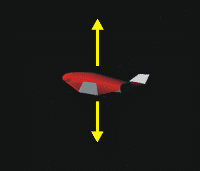
\includegraphics[width=0.3\textwidth, margin=0pt 1ex 0pt 1ex, valign=m]{control_up_down.png}
	\\
	\hline\rule{0pt}{2ex}
		\begin{itemize}[leftmargin=*]
		\item \keystroke{6}$_{Num}$ / \keystroke{9}$_{Num}$
		\end{itemize}
	&
		\begin{itemize}[leftmargin=*]
		\item \keystroke{1}$_{Num}$ / \keystroke{3}$_{Num}$
		\item Joystick rudder control
		\item Joystick left/right+Button 2
		\end{itemize}
	&
		\begin{itemize}[leftmargin=*]
		\item \keystroke{2}$_{Num}$ / \keystroke{8}$_{Num}$
		\item Joystick forward/back
		\end{itemize}
	\\
	\hline
	\end{tabular}
\end{table}

\noindent
For fine control of attitude thrusters with the keyboard use \Ctrl-Numpad key combinations. This engages the engines at 10\% thrust.\\
An important control function is the automatic \textit{Kill rotation} mode (\keystroke{5}$_{Num}$). This function fires appropriate attitude thrusters to stop the vessel's rotation. This mode remains active until the vessel's angular velocity is cancelled or until manually disengaged with another \keystroke{5}$_{Num}$.


\end{document}
